% HARPO — independent preprint (Zenodo / arXiv).
% Converted 2026-07-02 from the FPT'26 Track-A 2-page submission: the former
% appendices are now the body sections; de-anonymized; related work added.
% Build locally via Docker (see paper/README.md):
%   docker run --rm -v "$PWD":/work -w /work texlive/texlive:latest \
%     latexmk -pdf -interaction=nonstopmode -halt-on-error paper.tex
%
% Every quantitative claim is copied verbatim from docs/ablations/canonical/TABLE.md
% (the single source of truth) via docs/RESULTS.md / docs/PAPER.md. Do not edit numbers here.
\documentclass[conference]{IEEEtran}
\IEEEoverridecommandlockouts
\usepackage{cite}
\usepackage{amsmath,amssymb,amsfonts}
\usepackage{booktabs}
\usepackage{graphicx}
\usepackage{tikz}
\usetikzlibrary{arrows.meta,positioning,shapes.geometric,fit,backgrounds,calc}
\usepackage{url}
\usepackage{xcolor}
\usepackage[hidelinks]{hyperref}

\begin{document}

\title{HARPO: A Budget-Aware Repair-Then-Optimize\\Agent for HLS C/C++%
\thanks{Preprint v2, August 2026. Revises the July 2026 v1
(\url{https://doi.org/10.5281/zenodo.21366536}): this version withdraws several
unsupported claims, labels the pre-fix records as such, and adds a post-route
fidelity check (\S\ref{app:coverage:implverify}). Source code and the committed
canonical evidence behind every reported number:
\url{https://github.com/phucducnguyen/harpo}.}}

\author{\IEEEauthorblockN{Phuc (Patrick) Duc Nguyen}\\
\IEEEauthorblockA{Independent Researcher\\
pnguyen2101@gmail.com\\
ORCID: \href{https://orcid.org/0009-0000-6536-214X}{0009-0000-6536-214X}}}

\maketitle

\begin{abstract}
HARPO is a budget-aware autonomous agent for High-Level Synthesis (HLS) that first
\emph{repairs} a broken C/C++ kernel to functional correctness and then \emph{optimizes}
for quality of results (QoR)---performance and resource utilization, not power---under a strict per-task tool-invocation budget. It
runs as a closed control loop---run tool, parse report, diagnose, propose one minimal
change, verify, keep or roll back---not as a one-shot prompt, and it enforces
correctness before QoR: a candidate must pass C-simulation before any synthesis metric
can improve its rank.

Our central finding is that, in budgeted LLM4HLS, the deeper risk is not merely whether
the LLM writes \emph{correct} code, but whether the agent optimizes the \emph{right
hardware objective}. A raw LLM can over-parallelize, buying a 2$\times$ throughput gain
at order-of-magnitude area cost. We contribute three decision-policy fixes: (1)~a
\emph{metric} fix that scores throughput on the design \texttt{interval\_max} rather
than a per-loop initiation interval that can vanish under full unroll; (2)~a
\emph{policy} fix whose default objective satisfices throughput to a target and then
minimizes area; and (3)~an \emph{autonomy} fix---a zero-token, capped probe that
derives the throughput target when a task gives none.

We evaluate HARPO on real Vitis HLS~2025.2 targeting \texttt{xc7z020}, with a
local free model and a deterministic recipe baseline. All reported QoR figures are
csynth \emph{estimates}; a committed post-route check on 12 candidates observes a
LUT estimate error of 1.60--2.73$\times$ and is reported as a threat to validity.
That range is not a bound: the 12 candidates are those that passed the estimate
gate, so designs the gate excluded are unrepresented, and a case-study baseline
excluded at 168.7\% estimated LUT measures 3.47$\times$.
The corrected-objective
results are regenerable from the committed canonical evidence table
(\texttt{docs/ablations/canonical/}) and the scripts that produce it; the
historical pre-fix ablations are backed by committed per-run JSON under
\texttt{docs/ablations/}, and the aggregate suite table is regenerated locally
(\texttt{runs/} is not committed).
Across the demonstrated suite, 140 unit tests pass and the agent runs at \$0 LLM
API cost.
\end{abstract}

\begin{IEEEkeywords}
High-Level Synthesis, LLM agents, design-space exploration, budgeted optimization, FPGA.
\end{IEEEkeywords}

\section{Introduction}
High-Level Synthesis turns C/C++ into RTL, but reaching good QoR still demands expert
iteration over pragmas and code structure. A natural question is whether an
\emph{autonomous LLM agent} can do that iteration: interpret a task, repair or optimize
HLS code, invoke tool feedback, parse reports, prioritize correctness before QoR, and
\emph{terminate within a strict tool-invocation budget}. This problem setting---budgeted
LLM4HLS with a correctness-dominated ranking rule---follows the task formulation of the
FPT'26 AMD FPGA Design Competition, Track~A (LLM4HLS); HARPO was built independently
against that formulation, and this preprint reports the system and its evidence as
standalone research.

HARPO is such an agent. Beyond engineering the loop, our work isolates a subtle but
decisive failure mode: when an LLM is free to add pragmas greedily under a naive score,
it \emph{over-parallelizes}---on \texttt{mac8}, under our \emph{pre-fix} objective, it
once bought a 2\(\times\) throughput gain (interval 128 vs.\ 256) at \textbf{13194~LUT}
versus a deterministic recipe's \textbf{315~LUT} (\(\sim\)42\(\times\) the LUT;
\(\sim\)35\(\times\) the normalized \texttt{area\_score} the ranking consults), both
functionally correct. We show this is fundamentally a \emph{scoring} problem, not a
prompting problem, and fix it with three small, named changes to the agent's
decision-making (Sec.~\ref{app:scoring}). The contributions are:
\begin{itemize}
  \item a budget-aware repair-then-optimize agent with a \emph{structural}
    correctness-before-QoR guarantee (Sec.~\ref{app:arch});
  \item three decision-policy fixes---metric, policy, and autonomy---each motivated by a
    concrete, measured failure and re-baselined on real Vitis (Sec.~\ref{app:scoring});
  \item an honest, replayable recipe-vs-LLM ablation showing where a deterministic
    precise-pragma library beats a raw LLM and where it cannot reach
    (Secs.~\ref{app:scoring} and~\ref{app:results});
  \item full results under synthesis estimates, a post-route fidelity check, an
    honest task-coverage map, and a \$0-cost local-only replay recipe
    (Secs.~\ref{app:results}, \ref{app:coverage}, and~\ref{app:repro}).
\end{itemize}

\section{Related Work}
\label{sec:related}
Pragma-level design-space exploration long predates LLMs: HLS surveys catalogue the
gap between naive C and expert-tuned kernels~\cite{nane2016survey}, and search-based
tools such as AutoDSE~\cite{autodse} treat pragma insertion as a bottleneck-guided
optimization problem. HARPO's deterministic recipe library is a deliberately
minimal member of this family---a catalogue of exact, correct-by-construction pragmas
rather than a search---used here both as a provider and as an ablation baseline.

More recently, LLMs have been applied across the HLS flow: refactoring software C
into synthesizable C (C2HLSC~\cite{c2hlsc}), LLM-driven end-to-end flows with
profiling and DSE (HLSPilot~\cite{hlspilot}, ChatHLS~\cite{chathls}), fine-tuned
pragma insertion (LIFT~\cite{lift}), LLM-guided design-space exploration
(iDSE~\cite{idse}), and benchmarks for evaluating LLMs on HLS design tasks
(HLS-Eval~\cite{hlseval}). These works largely target design \emph{quality} or
\emph{coverage} given generous tool access.

A concurrent wave (2025--2026) makes the agentic framing explicit: general-purpose
coding agents optimizing HLS kernels (Agent Factories~\cite{agentfactorieshls}),
self-evolving agentic refactoring for HLS compatibility and performance
(AgRefactor~\cite{agrefactor}), QoR-aware code generation via reinforcement learning
with a proxy reward (HLS-Seek~\cite{hlsseek}), evidence-driven multi-agent
C-to-synthesizable-C conversion and verification~\cite{evidencedrivenhls},
timing-aware architecture-specific optimization (TimelyHLS~\cite{timelyhls}), and
LLM-based HLS logic-bug repair (HLSDebugger~\cite{hlsdebugger}). These share HARPO's
agentic loop but optimize for raw quality or coverage, typically with generous tool
access and often frontier models; none makes a strict per-task \emph{tool-invocation
budget} the governing constraint, nor isolates the scoring-function failure mode we
study.

HARPO differs in three ways. First, the \emph{tool-invocation budget} is a
first-class constraint: every csim, csynth, and LLM call is metered, gated by policy,
and reported. Second, correctness-before-QoR is \emph{structural}, not advisory: an
optimization's synthesis metrics are never even read until the candidate re-passes
C-simulation. Third, rather than showcasing the LLM, we ablate it honestly against a
zero-token deterministic baseline and find that under a naive score the LLM's fluency
is not the binding risk---the \emph{objective} is. All of this runs on a small local
model at \$0 API cost, whereas most prior work relies on frontier commercial models.

% ===================== BODY SECTIONS (former appendices) =====================
\section{The HARPO Agent}\label{app:arch}

HARPO normalizes a task bundle (\texttt{spec/constraints/budget} JSON)
into one \texttt{TaskContext}---top function, sources, testbench, part,
clock, policy, budget---all \emph{injected}, never hardcoded, so the same
agent runs an external evaluator's tasks unchanged. A tool runner
dispatches stages to a backend: host \texttt{g++} (functional csim, since
g++ ignores \texttt{\#pragma HLS}) or \texttt{vitis\_hls} (real
csim+csynth). A deterministic report parser maps logs to typed statuses; a
rule-based diagnosis engine maps a status to an action. Patch providers
share one protocol with three implementations: \texttt{recipe} (a
deterministic precise-pragma library, 0~tokens), \texttt{ollama} (a local
LLM), and \texttt{mock} (for tests). The two loops are \emph{repair} (csim
$\rightarrow$ diagnose $\rightarrow$ patch $\rightarrow$ re-csim) and
\emph{optimize} (baseline csim+csynth $\rightarrow$ propose pragma
$\rightarrow$ apply $\rightarrow$ re-verify csim $\rightarrow$ csynth
$\rightarrow$ keep iff the score strictly improves); \texttt{pipeline}
chains them on one shared budget.

In detail, HARPO is built from six cooperating components and two
control loops, chained by a pipeline that runs on a single shared per-task
budget account. This section details each component, the operational
steps of each loop, the \texttt{BudgetManager} that meters all tool
calls, the correctness-dominated lexicographic score, and the
correctness-preserving invariant that makes ``correctness before PPA''
structural rather than advisory.

\subsection{The six components}\label{app:arch:components}

\begin{enumerate}
  \item \textbf{Task loader.} Normalizes a task bundle
    (\texttt{spec.json} + \texttt{constraints.json} +
    \texttt{budget.json}) into one \texttt{TaskContext}: top function,
    source/testbench file lists, part, clock, policy, and budget. Part,
    clock, and sources are \emph{injected}, never hardcoded, so the same
    agent runs the evaluator's tasks unchanged.
  \item \textbf{Tool runner.} Dispatches a stage to a backend:
    \texttt{gpp} (host g++ compile+run = functional csim, no Vitis
    needed, since g++ ignores \texttt{\#pragma HLS}) or
    \texttt{vitis\_hls} (real csim+csynth via a generated
    \texttt{run\_harpo.tcl}).
  \item \textbf{Report parser.} \texttt{parse\_csim} $\rightarrow$
    \{pass, compile\_error, functional\_fail, timeout,
    tool\_unavailable\}; \texttt{parse\_csynth} $\rightarrow$ II, depth,
    latency best/worst, Fmax, LUT/FF/DSP/BRAM + util\% from the Vitis
    XML, with timing/resource violations.
  \item \textbf{Diagnosis engine.} Rule-based and deterministic (no
    model): maps a parsed status to a recommended action. A
    clean/improvable csynth pass yields \texttt{optimize\_ppa}; a
    repeated failure escalates to \texttt{rollback\_or\_escalate}.
  \item \textbf{Patch providers.} A uniform \texttt{PatchProvider}
    protocol with three implementations: \texttt{mock} (deterministic
    string edits, for tests/demo), \texttt{recipe} (deterministic
    precise-pragma library, no tokens), and \texttt{ollama} (local LLM
    over stdlib \texttt{urllib}, never raises---degrades to the next
    provider). Each reports \texttt{last\_usage} tokens.
  \item \textbf{Candidate store + lexicographic score.} Every attempt
    is an isolated, forkable copy of the source; the edited kernel is
    compiled against the \emph{un-edited} testbench; the winner is
    whichever candidate scores highest. The \texttt{BudgetManager} is
    the budget spine (per-tool limits + reserve + policy gates).
\end{enumerate}

\subsection{The two control loops}\label{app:arch:loops}

The agent runs two loops over the candidate store. The repair loop
restores correctness; the optimize loop improves power, performance, and
area (PPA) without ever breaking correctness. Rendered as step
sequences rather than a wide ASCII diagram, they are as follows.

\subsubsection{Repair loop (correctness)}
\begin{enumerate}
  \item Run csim via \texttt{gpp}, parse the report, and diagnose.
  \item If csim passes, stop: the current candidate is the winner
    (DONE).
  \item Otherwise check \texttt{budget.policy\_allows(llm)}.
  \item If allowed, call \texttt{provider.propose()} in provider order
    (\texttt{recipe} $\rightarrow$ \texttt{ollama}), accumulating
    tokens.
  \item Run \texttt{check\_contract} (signature / testbench / globals).
  \item If the contract holds, fork the source, apply the patch, and
    loop back to step~1.
  \item Stop on any of: csim pass; \texttt{max\_steps} reached; budget
    exhausted; or a repeated/regressed state.
\end{enumerate}

\subsubsection{Optimize loop (PPA, never breaks correctness)}
\begin{enumerate}
  \item Require the baseline csim to pass; otherwise return ``run repair
    first.''
  \item Run the baseline csynth to obtain \texttt{baseline\_metrics}.
  \item Loop while \texttt{steps < max} and
    \texttt{no\_improve < patience}:
  \begin{enumerate}
    \item \texttt{diagnose\_csynth} $\rightarrow$
      \texttt{provider.propose()}.
    \item \texttt{check\_contract}; fork; \texttt{apply\_patch}.
    \item \textbf{Re-verify csim} on the forked candidate; if it broke
      functional behavior, DISCARD the candidate.
    \item If csim still passes, run \texttt{csynth(child)}.
    \item Compute \texttt{score(child)}; if it is strictly greater than
      \texttt{score(best)}, ACCEPT, else REJECT.
  \end{enumerate}
\end{enumerate}

\subsubsection{Pipeline}
\texttt{run\_pipeline} chains repair then optimize on \textbf{one}
shared per-task \texttt{BudgetManager}, so repair and optimize debit the
same account.

\subsection{BudgetManager (the budget spine)}\label{app:arch:budget}

The \texttt{BudgetManager} is constructed from \texttt{budget.json}
(\texttt{mode: per\_tool}). Its per-tool limits are
\texttt{\{static\_check:100, csim:20, csynth:10, cosim:5,
llm\_calls:30\}}, with a held-back \texttt{reserve
\{final\_csim:1, final\_csynth:1, final\_cosim:1\}}. A missing limit is
unlimited. \texttt{can(action)} is true only while
$\texttt{spent} < \texttt{limit} - \texttt{reserve}$---the reserve
guarantees a winner can always be re-verified at the end.

\texttt{policy\_allows} enforces three gates, in order:
\begin{enumerate}
  \item \textbf{Budget} --- \texttt{can(action)} must hold before the
    call.
  \item \textbf{Stage ordering} --- no csynth/cosim before csim passes.
  \item \textbf{Stop/rollback guard} --- refuse another LLM call when
    the state is \emph{repeated} or \emph{regressed}.
\end{enumerate}

These ``don't-waste rules'' make tool calls---the scarce resource the
setting meters---the budgeted quantity: no csynth before csim
passes, and no fresh LLM call when re-trying a failing fix would burn
budget for nothing. The four demonstrated tasks of Sec.~\ref{app:suite} spent
\textbf{42 tool calls} and \textbf{2400 tokens} total---comfortably inside the
per-task limits (csim~20, csynth~10, llm\_calls~30).

\subsection{The correctness-dominated lexicographic score}\label{app:arch:score}

Ranking proceeds top-down so that correctness dominates PPA:
\begin{enumerate}
  \item \textbf{Correctness tier} --- 0: csim unknown/fail; 1: csim
    pass; 2: csim+csynth pass. A tier-2 candidate always outranks a
    tier-1, regardless of PPA.
  \item \textbf{Throughput on the design \texttt{interval\_max}} (within
    a tier) --- \emph{not} the per-loop II, which is diagnostic-only.
  \item \textbf{Objective-dependent secondary order.} The default
    objective is \texttt{satisfice\_then\_area}: once a candidate meets
    the per-task \texttt{throughput\_target} it is ranked by lowest
    normalized \texttt{area\_score}, then ADP (area $\times$ interval).
\end{enumerate}

The other objectives (\texttt{speed\_first}, \texttt{area\_first},
\texttt{adp}, \texttt{pareto\_report}) reorder these terms. The old
II-first, latency, LUT lexicographic order is no longer the live score;
ranking II ahead of latency is the right default for
streamed/throughput kernels but can \emph{raise single-call latency}
(on \texttt{matmul\_001}, \texttt{latency\_worst} rose
$260 \rightarrow 518$ even as II improved $4 \rightarrow 1$, because the
loop greedily takes the initiation-interval win), which is why the
per-task objective knob exists.

\subsection{The correctness-preserving invariant}\label{app:arch:invariant}

An optimization is accepted only if it (a)~still passes csim AND
(b)~strictly improves the score. Every forked candidate is re-run
through csim \emph{before} its csynth metrics are read; if a pragma
broke functional behavior, the candidate is discarded and its metrics
are never trusted. This is the structural guarantee behind
``correctness before PPA'': the agent can never trade a wrong-but-fast
design up the ranking. The invariant is proven by a hermetic test,
\texttt{tests/test\_optimize\_safety.py} with
\texttt{tasks/trap\_breakscsim\_001}; \textbf{106 unit tests} total, all
green.

\section{Scoring Overhaul and Recipe-vs-LLM Analysis}\label{app:scoring}

This section develops the paper's central contribution: why a
deterministic recipe library beats a raw LLM on structured-reduction kernels, why
the area blow-up of the LLM arm was ultimately a \emph{scoring} defect rather than a
prompting defect, and how two distinct fixes (plus an autonomy probe) make the
elegant recipe outrank the LLM under honest scoring. All numbers are copied verbatim
from the committed canonical evidence under \texttt{docs/ablations/canonical/} (the raw
\texttt{runs/} tree is gitignored and regenerated locally), with one deliberate
exception: figures drawn from the \emph{pre-fix} run record that motivated the overhaul
(\texttt{docs/ablations/mac8\_001\_ollama.json}) --- the raw-LLM row of
Table~\ref{tab:headline} and the within-run rescoring in \S\ref{app:scoring:cause}.
Those are flagged as pre-fix wherever they appear. Normalized \texttt{area\_score}
values quoted below are recomputed from the stored csynth metrics via
\texttt{harpo/area.py}; the run logs store raw resource counts, not the score.
The canonical 21-row evidence table is \texttt{docs/ablations/canonical/TABLE.md},
regenerable via \texttt{scripts/ablation\_table.py}.

\subsection{The recipe library}\label{app:scoring:recipes}

The deterministic \textbf{recipe library} (\texttt{recipes.py}) emits
\emph{fully specified} HLS pragmas, one per call, by robust
text scanning (\texttt{ARRAY\_PARTITION cyclic factor=N dim=1},
\texttt{PIPELINE II=1}, \texttt{UNROLL factor=N}, \ldots). An offline g++ self-test checks that each emitted kernel is
valid C++ (g++ ignores \texttt{\#pragma HLS}, so this checks the surrounding code,
not the pragma's HLS effect); the pragmas themselves are exercised end-to-end on
real Vitis in the ablations below. It costs \textbf{0 tokens}. The optimize default
provider order is \texttt{recipe,ollama} --- precise deterministic recipes first, the
LLM only for the tail the catalogue cannot reach (``dumbest reliable tool first'').

\subsection{The headline mac8 ablation}\label{app:scoring:headline}

Table~\ref{tab:headline} reports the headline ablation
(\texttt{docs/ablations/recipe-vs-llm.md}): the same optimize loop, the same kernel
\texttt{mac8\_001}, two providers, real Vitis HLS 2025.2.

\begin{table}[h]
\centering\small
\caption{Headline \texttt{mac8\_001} ablation: recipe vs.\ raw LLM, real Vitis HLS
2025.2 --- csynth estimates, not post-place-and-route measurements. The
\texttt{ollama-best} row is a \textbf{historical pre-fix record}; see note~2.}
\label{tab:headline}
\begin{tabular}{lrrrrrr}
\toprule
design & II & latency & interval & LUT & FF & tokens \\
\midrule
baseline      & 4   & 1026 & 1024 & 369        & 153 & --- \\
recipe-best   & \textbf{1} & 259  & 256  & \textbf{315}   & 126 & \textbf{0} \\
ollama-best$^{2}$ & n/a$^{1}$ & \textbf{129} & 128  & \textbf{13194} & 322 & \textbf{34387} \\
\bottomrule
\end{tabular}

\vspace{2pt}
{\footnotesize $^{1}$ The LLM fully unrolls the outer loop, so Vitis reports no
per-iteration II (\texttt{ii: null}); throughput shows as total interval 128
(vs.\ baseline 1024) --- a real, correct throughput win, paid for in area. Both arms
re-verified csim-correct. The recipe-best move was a single
\texttt{ARRAY\_PARTITION cyclic factor=8 dim=1}; the LLM stacked
partition$\times$2 + \texttt{PIPELINE II=1} + \texttt{UNROLL factor=8}.\par
$^{2}$ \textbf{Pre-fix provenance.} This row was produced under the \emph{old} score
(per-loop II, then latency, with area last) --- the defect this section diagnoses ---
and is preserved in \texttt{docs/ablations/mac8\_001\_ollama.json}, outside
\texttt{docs/ablations/canonical/}. The baseline and \texttt{recipe-best} rows are
objective-invariant and reproduce unchanged in the canonical table. Under the
corrected objective the raw-LLM arm on this kernel improves nothing and keeps the
369-LUT baseline at 7207 tokens (Table~\ref{tab:recipe-vs-llm}). That is a
\emph{different run with a different trajectory}, not this one rescored: it stops
after two rejected candidates when the patience limit trips, and the 13194-LUT design
was never regenerated post-fix.}
\end{table}

This is \textbf{$\sim$42$\times$ the LUT for 2$\times$ the throughput} (recipe 315 LUT at
interval 256 vs.\ LLM 13194 LUT at interval 128; the LLM is also lower-latency, 129
vs.\ 259). On the normalized \texttt{area\_score} the ranking actually consults
(\S\ref{app:scoring:fixes}) the gap is $\sim$35$\times$ (0.0071 vs.\ 0.2510); the LUT
ratio is the larger of the two because this design's FF growth is small against the
device's FF capacity. For \texttt{xc7z020} (53{,}200 LUT) the recipe sits at 0.6\% LUT
utilization, the LLM design at 24.8\%. We note explicitly that the LLM arm's throughput win is
real: the failure is not that it bought nothing, but that the score let it pay two
orders of magnitude of area for a factor of two. The committed repeat files for this
arm (\texttt{\_run1/2/3.json}) are byte-identical to one another, and decoding is
greedy (temperature 0), so they evidence \emph{replayability} rather than run-to-run
stability; cross-run variance was not measured.

\subsection{The honest corrected cause: over-parallelization, enabled by the score}\label{app:scoring:cause}

A prior note framed the blow-up as an \emph{imprecise} \texttt{ARRAY\_PARTITION}
(missing the partition type) defaulting to \texttt{complete}. With the current
optimizer prompt (\texttt{\_OLLAMA\_OPT\_SYSTEM\_PROMPT}, which forbids bare
\texttt{ARRAY\_PARTITION} and warns that omitting the type ``detonates area'') the LLM
no longer makes that mistake --- every partition it emitted was a fully-specified
\texttt{cyclic factor=N}. The area blow-up \textbf{reproduced anyway, via a different
mechanism}: the LLM stacks \texttt{PIPELINE II=1} \emph{plus} \texttt{UNROLL factor=8}
on top of partitioning, fully spatially unrolling the reduction. Each step strictly
improves the lexicographic score (II $\rightarrow$ latency dominate area), so the
greedy loop accepts the ever-larger-but-faster design. The lesson, sharpened: a raw
LLM is fluent but imprecise about \emph{how hard to push} --- it over-applies
parallelism for marginal latency at order-of-magnitude area cost, while the recipe
applies exactly the one pragma that unblocks II=1 and stops.

Crucially, a follow-up re-ablation traced the \emph{enabler} of the blow-up to the
\textbf{score itself}, not the LLM. A fully-unrolled loop reports no per-loop II
(\texttt{None}), which the old throughput term sorted as neutral and thus ranked
\emph{above} a real II$\geq$1 --- so the loop literally rewarded over-unrolling (it
even accepted a design with interval 3073 vs.\ the baseline's 1024). Prompt hardening
alone does not fix this. Both durable fixes (\S\ref{app:scoring:fixes}) are now
implemented. Fig.~\ref{fig:scoring} contrasts the two scoring regimes and the ranking
the corrected objective implies.

The same committed run record also carries a rescoring result that needs no
cross-run comparison at all, and it is the sharpest evidence we have.
\texttt{docs/ablations/mac8\_001\_ollama.json} stores every candidate with its csynth
metrics and its pre-fix score tuple. Two of them share an identical design
\texttt{interval\_max} of 128: \texttt{cand\_0004} at \textbf{13194~LUT}
(\texttt{ii: null}) scored $(2,0,-129,-13194,0)$, and \texttt{cand\_0005} at
\textbf{1092~LUT} (\texttt{ii}~=~4) scored $(2,-4,-131,-1092,0)$. The old score kept
\texttt{cand\_0004} --- 12$\times$ the LUT and 10.7$\times$ the normalized
\texttt{area\_score} (0.2510 vs.\ 0.0235) --- for a 1.5\% latency edge (129 vs.\ 131
cycles) and \emph{no throughput gain whatsoever}, purely because a missing per-loop II
sorted as neutral and outranked a real \texttt{ii}~=~4. Re-scoring that same realized
candidate pool under \texttt{interval\_max}~+~\texttt{satisfice\_then\_area} (target
256) selects \texttt{cand\_0005}. This is a rescoring of one run's own candidates, not
a re-run: a corrected-objective run would have proposed differently, as the canonical
LLM arm in fact did (Table~\ref{tab:recipe-vs-llm}).

\begin{figure}[t]
\centering
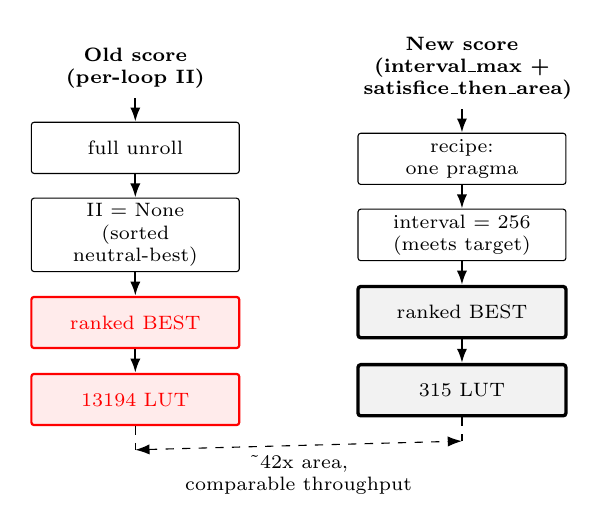
\begin{tikzpicture}[
  font=\scriptsize,
  node distance=3mm,
  htitle/.style={align=center, font=\scriptsize\bfseries, text width=2.5cm},
  block/.style={draw, rounded corners=1pt, align=center, inner sep=2pt,
                minimum height=0.65cm, text width=2.5cm},
  badblock/.style={block, draw=red, thick, fill=red!8, text=red},
  goodblock/.style={block, draw=black, very thick, fill=black!5},
  arrow/.style={-{Latex[length=1.8mm,width=1.3mm]}, thick}
]

% left column: old per-loop-II score
\node[htitle] (Lh) {Old score\\(per-loop II)};
\node[block, below=of Lh] (L2) {full unroll};
\node[block, below=of L2] (L3) {II = None\\(sorted neutral-best)};
\node[badblock, below=of L3] (L4) {ranked BEST};
\node[badblock, below=of L4] (L5) {13194 LUT};

\draw[arrow] (Lh.south) -- (L2.north);
\draw[arrow] (L2.south) -- (L3.north);
\draw[arrow] (L3.south) -- (L4.north);
\draw[arrow] (L4.south) -- (L5.north);

% right column: corrected score
\node[htitle, right=1.4cm of Lh] (Rh) {New score\\(interval\_max +\\satisfice\_then\_area)};
\node[block, below=of Rh] (R2) {recipe:\\one pragma};
\node[block, below=of R2] (R3) {interval = 256\\(meets target)};
\node[goodblock, below=of R3] (R4) {ranked BEST};
\node[goodblock, below=of R4] (R5) {315 LUT};

\draw[arrow] (Rh.south) -- (R2.north);
\draw[arrow] (R2.south) -- (R3.north);
\draw[arrow] (R3.south) -- (R4.north);
\draw[arrow] (R4.south) -- (R5.north);

% comparison between the two final outcomes
\draw[dashed] (L5.south) -- ++(0,-0.3cm) coordinate (Lb);
\draw[dashed] (R5.south) -- ++(0,-0.3cm) coordinate (Rb);
\draw[{Latex[length=1.8mm,width=1.3mm]}-{Latex[length=1.8mm,width=1.3mm]}, dashed]
  (Lb) -- (Rb) node[midway, below, font=\scriptsize, align=center]
  {\textasciitilde42x area,\\comparable throughput};

\end{tikzpicture}
\caption{Why scoring, not prompting, was load-bearing (\texttt{mac8\_001}). Under the old per-loop-II metric a fully-unrolled design reports II=None, sorted as neutral-best, so the greedy loop rewards over-unrolling to 13194 LUT. Under the corrected metric (design \texttt{interval\_max}) plus the \texttt{satisfice\_then\_area} objective, the elegant single-pragma recipe design (315 LUT) outranks it. Same loop, same LLM; the ranking inverts.}
\label{fig:scoring}
\end{figure}


\subsection{The two fixes, in depth}\label{app:scoring:fixes}

The over-parallelization enabler is \textbf{two distinct defects} with \textbf{two
distinct fixes}, both implemented and re-baselined on real Vitis (136/136 unit tests
green).

\paragraph{Fix 1 --- metric: throughput is scored on the design \texttt{interval\_max}, not the per-loop \texttt{PipelineII}.}
The per-loop term sorted a fully-unrolled loop's missing II (\texttt{None}) as neutral
0, beating a real II$\geq$1 and rewarding over-unrolling. \texttt{interval\_max} is
always reported by Vitis; per-loop \texttt{ii} is now diagnostic-only. Under it, the
accepted \texttt{mac8\_001} interval-3073 design correctly loses to the baseline
(1024), and the old \texttt{conv2d\_001} over-pragma'd candidate (interval 328)
correctly loses to the baseline (191) --- while the proper recipe move now drives
conv2d to interval 82 under a target (\S\ref{app:scoring:rebaseline}).

\paragraph{Fix 2 --- policy: the default objective is \texttt{satisfice\_then\_area}.}
The per-task objective is a 5-value enum --- \texttt{speed\_first}, \texttt{area\_first},
\texttt{adp}, \texttt{satisfice\_then\_area} (default), \texttt{pareto\_report}
(\texttt{spec.json} \texttt{objective}; legacy \texttt{throughput}/\texttt{latency}
alias to \texttt{speed\_first}; unknown/absent $\rightarrow$ default).
\texttt{interval\_max} scoring alone does not stop a \emph{genuinely faster but huge}
design from winning on throughput; satisficing throughput to a per-task
\texttt{throughput\_target} and then minimizing area is what would make the elegant recipe
(interval 256 / 315 LUT) outrank the LLM blow-up (128 / 13194 LUT) were both offered to
one loop: with \texttt{throughput\_target}~=~256 both meet the target, so the next key is
area, and \texttt{area\_score} 0.0071 beats 0.2510. That is a property of the objective
(\texttt{harpo/candidate.py}) evaluated on the two committed designs rather than an
observed head-to-head --- the pre-fix blow-up was never regenerated under the corrected
objective (note~2 of Table~\ref{tab:headline}). The within-run rescoring in
\S\ref{app:scoring:cause} is the observed counterpart.

Supporting these, a new \texttt{harpo/area.py} provides a normalized
\texttt{area\_score} (used/available summed over LUT/FF/DSP/BRAM, with \emph{no
per-resource weights} so scarcity is not double-counted; per-part fallback for
xc7z020), \texttt{adp = area\_score $\times$ interval\_max}, and two reporting
helpers not consulted by the ranking (\texttt{resource\_growth\_ratio},
\texttt{pareto\_front}). A new per-task
\texttt{throughput\_target} field carries the \texttt{interval\_max} ceiling the
satisfice policy targets.

\paragraph{Fix 3 --- autonomy: a recipe-only capped probe derives the target when the task gives none.}
\texttt{satisfice\_then\_area} needs a \texttt{throughput\_target}; rather than require
a hand-written one, \texttt{harpo/probe.py} derives it. The probe is deliberately
minimal: \textbf{recipe-only, zero LLM tokens}, capped at \texttt{max\_synth}
single-pragma forks from the baseline (default 4), \textbf{full unroll excluded}. The
target is the lowest \texttt{interval\_max} among the baseline and any probe candidate
that csim+csynth-passes \emph{and} stays within \texttt{area\_score} $\leq$ 2$\times$
baseline; if nothing beats the baseline within that cap, it falls back to the baseline
\texttt{interval\_max} (never an unreachable goal). On \texttt{mac8\_001} with its
target stripped, the probe derives \textbf{256} --- exactly the hand-set value --- at
0 tokens.

\subsection{Re-baseline under the new scoring}\label{app:scoring:rebaseline}

Recipe arm, real Vitis 2025.2, \texttt{xc7z020clg400-1}, 10 ns. Every number here is a
row in the canonical evidence table (\texttt{docs/ablations/canonical/TABLE.md}). The
two fixes show on two kernels.

\paragraph{\texttt{mac8} (Fix 1, metric).} Full unroll makes \texttt{interval\_max}
\emph{worse} (3073) $\rightarrow$ Fix 1 discards it, and the recipe reaches interval
256 / LUT 315.

\paragraph{\texttt{matmul} (Fix 2, policy).} Full unroll makes \texttt{interval\_max}
genuinely \emph{better}, so the metric fix alone will not stop it. The two matmul
recipe rows make the case directly (Table~\ref{tab:matmul}):
\texttt{speed\_first} reaches interval 19 / LUT 5689 / FF 14999 (area\_score 1.121,
ADP 21.292), while \texttt{satisfice\_then\_area} (target 72) keeps interval 44 /
LUT 3121 / FF 5932 (area\_score 0.3326, ADP 14.6344) --- $\sim$45\% fewer LUT,
$\sim$60\% fewer FF, \emph{and} a lower ADP, for 25 cycles of interval. The target is
what governs the over-push.

\begin{table}[h]
\centering\small
\caption{\texttt{matmul\_001} recipe arm: \texttt{satisfice\_then\_area} (target 72) vs.\ \texttt{speed\_first}.}
\label{tab:matmul}
\resizebox{\columnwidth}{!}{%
\begin{tabular}{lrrrrr}
\toprule
policy & interval & LUT & FF & area\_score & ADP \\
\midrule
baseline                & 256 & 706  & 579   & 0.04599 & 11.7722 \\
satisfice (target 72)   & 44  & \textbf{3121} & \textbf{5932}  & 0.3326  & \textbf{14.6344} \\
speed\_first            & \textbf{19} & 5689 & 14999 & 1.121   & 21.292 \\
\bottomrule
\end{tabular}}
\end{table}

\paragraph{PolyBench (Fix 3, probe).} Three PolyBench kernels (gemm/atax/bicg, integer
16$\times$16) extend the evidence beyond hand-built toys; all three auto-derive their
target via the Fix-3 probe (Table~\ref{tab:polybench}). \texttt{gemm} conservatively
falls back to baseline 2060 (no improvement, baseline kept); \texttt{atax} derives a
real target of 280 and reaches interval 64 / LUT 3907; \texttt{bicg} derives 162 and
reaches interval 60 / LUT 3596. One scoping note, since it is easy to read the probe's
cap as a guarantee: the 2$\times$ \texttt{area\_score} cap governs \emph{target
derivation} only. In both kernels the design the optimize loop ultimately kept is the
same array partition the probe had excluded at that cap --- 3.54$\times$ baseline
\texttt{area\_score} for \texttt{atax}, 4.89$\times$ for \texttt{bicg} (on raw LUT the
same two designs are only 1.57$\times$ and 1.66$\times$; the growth is DSP-driven,
12$\rightarrow$96 on \texttt{bicg}). Once the target is set, the satisfice policy
bounds \emph{throughput}, not area.

\begin{table}[h]
\centering\small
\caption{PolyBench recipe arm (16$\times$16 integer), targets auto-derived by the Fix-3 probe.}
\label{tab:polybench}
\resizebox{\columnwidth}{!}{%
\begin{tabular}{llrrrr}
\toprule
kernel & target & interval & LUT & FF & ADP \\
\midrule
gemm\_001 & 2060 (fallback)     & 2060 & 1238 & 1180 & 126.965 \\
atax\_001 & 280 (auto-derived)  & 64   & 3907 & 5596 & 22.0298 \\
bicg\_001 & 162 (auto-derived)  & 60   & 3596 & 8929 & 35.2726 \\
\bottomrule
\end{tabular}}
\end{table}

\subsection{Recipe-vs-LLM comparison under honest scoring}\label{app:scoring:comparison}

Table~\ref{tab:recipe-vs-llm} is the head-to-head, recipe vs.\ raw LLM under the
corrected scoring (the four re-baselined LLM arms). On structured-reduction kernels the
raw LLM over-parallelizes and, under the corrected scoring, \textbf{wins nothing}; the
precise recipe applies the single unblocking pragma. On kernels the safe recipes cannot
crack both are null; elsewhere they are comparable. The \texttt{recipe}-before-\texttt{ollama}
default is what captures the best of both.

\begin{table*}[t]
\centering\small
\caption{Recipe vs.\ raw LLM under honest (\texttt{interval\_max} + \texttt{satisfice\_then\_area}) scoring.}
\label{tab:recipe-vs-llm}
\begin{tabular}{llll}
\toprule
kernel & recipe arm & raw-LLM arm & winner \\
\midrule
mac8\_001   & interval 256 / LUT 315                          & no improvement (full-unroll interval 3073 discarded) & \textbf{recipe} \\
matmul\_001 & interval 44 / LUT 3121 \emph{(satisfice, target 72)} & no improvement (no candidate meets target)          & \textbf{recipe} \\
gemm\_001   & no improvement (probe fallback, target 2060)    & no improvement                                       & tie (both null) \\
atax\_001   & interval 64 / LUT 3907 / ADP 22.0               & interval 81 / LUT 3994 / ADP 28.0                    & recipe (marginal) \\
\bottomrule
\end{tabular}
\end{table*}

LLM-arm re-baselines for the remaining hand-built kernels, and additional PolyBench
ports, remain future work; the released evidence covers the four head-to-head kernels
above.

\paragraph{Fairness of the derived target.} The satisfice target in these
head-to-head rows comes from the Fix-3 probe, which is \emph{recipe-only}
(\S\ref{app:scoring:fixes}), and that same target then scores both arms. The probe
is the agent's autonomous fallback when a task ships no target, so using it here
matches how the agent runs in practice; even so, it lets the recipe arm help define
the objective the LLM arm is judged against. Two changes would make the comparison
fully neutral, and we leave both to future validation. An externally supplied
\texttt{throughput\_target}, of the kind a real evaluator provides, would keep either
arm from setting it. A target-sensitivity sweep---scaling the target across, say,
$1.0/0.75/0.5/0.25\times$ the probe value---would show whether the recipe-vs-LLM
ordering holds across operating points or is an artifact of one derived target. The
probe's selection rule is already provider-neutral (lowest \texttt{interval\_max}
within a $2\times$ area cap); what is open to question is where the candidates come
from.

\section{Full Synthesis-Estimate Results}\label{app:results}

This section collects the complete synthesis-estimate evidence behind the analysis of
Sec.~\ref{app:scoring} (all resource and timing numbers are Vitis HLS \emph{csynth
estimates}, not post-place-and-route measurements). Every number is copied verbatim from the
committed canonical ablation table (\texttt{docs/ablations/canonical/TABLE.md}),
which is generated, not hand-maintained, from real Vitis HLS 2025.2 runs on part
\texttt{xc7z020clg400-1} at a 10\,ns clock---or, for the pre-fix records
preserved below, from their (locally regenerated) pre-fix run logs (e.g.\ the \texttt{stencil3\_001}
best under the old objective keeps FF~54; the canonical table's FF~43 candidate
was rejected by that objective).

The numbers below use two different objectives, and the distinction matters. The
repair demonstration (\S\ref{app:repair}) does not depend on the objective at all.
The optimize kernels re-baselined under the current default (\texttt{interval\_max}
throughput with \texttt{satisfice\_then\_area}) are in Sec.~\ref{app:scoring:rebaseline}.
The before/after tables (\S\ref{app:ppa}, \S\ref{app:matmul}) and the full suite table
(\S\ref{app:suite}) instead keep their original numbers under the earlier lexicographic
objective, and each caption flags them as historical. Where a historical per-kernel
record disagrees with the canonical evidence table, the canonical table
(\texttt{docs/ablations/canonical/TABLE.md}) is authoritative.

\subsection{Repair Metrics}\label{app:repair}

Task \texttt{vadd\_buggy\_001} is a vector add with a planted wrong operator
(\texttt{c[i] = a[i] - b[i]}, should be \texttt{+}). The agent repaired it in two
steps with a single LLM call at \$0 cost (local model). Table~\ref{tab:repair}
reports the full repair metrics.

\begin{table}[h]
\centering
\small
\begin{tabular}{@{}ll@{}}
\toprule
Metric & Value \\
\midrule
Repaired & true (winner \texttt{cand\_0001}) \\
Steps & 2 \\
LLM calls & 1 \\
Tokens (prompt / completion / total) & 2054 / 346 / 2400 \\
Budget spent (csim / csynth / prop$^{\dagger}$) & 2 / 0 / 1 \\
Cost & \$0 (local model) \\
\bottomrule
\end{tabular}
\caption{Repair metrics for \texttt{vadd\_buggy\_001}: a one-character functional
fix found in a single local-LLM call at zero cost. $^{\dagger}$\texttt{prop} counts
provider \emph{proposals} (here one real LLM call), not tokens; recipe proposals cost
0 tokens.}
\label{tab:repair}
\end{table}

\subsection{Optimize QoR Before/After (historical, pre-fix objective)}\label{app:ppa}

The three 1-D reduction tasks were driven by the deterministic \texttt{recipe}
provider and spent zero LLM tokens. The winning move in every case was a cyclic
array partition on the kernel input that unblocked pipelining to II=1, kept only
when the candidate re-passed csim and strictly improved the score.
Table~\ref{tab:ppa} reports QoR before $\rightarrow$ after under the \emph{pre-fix}
lexicographic objective (the corrected-objective re-baseline of these kernels is in
Sec.~\ref{app:scoring:rebaseline}). \texttt{mac8\_001} gets
faster \emph{and} smaller, and \texttt{unroll8\_001} is the headline latency win
($\approx$7.8$\times$, 1026$\rightarrow$132) while also shrinking LUT and FF. For
\texttt{stencil3\_001} the LUT rose (193$\rightarrow$435) and Fmax fell, but II and
latency both improved; the (then-default) lexicographic score prioritizes II then
latency over LUT, so the design is correctly accepted under that objective.

\begin{table}[h]
\centering
\small
\resizebox{\columnwidth}{!}{%
\begin{tabular}{@{}lccccc@{}}
\toprule
Task & II & Latency (worst) & LUT & FF & Fmax (MHz) \\
\midrule
\texttt{mac8\_001}     & 4$\rightarrow$1 & 1026$\rightarrow$259 & 369$\rightarrow$315 & 153$\rightarrow$126 & 144.45$\rightarrow$144.45 \\
\texttt{stencil3\_001} & 2$\rightarrow$1 & 514$\rightarrow$259  & 193$\rightarrow$435 & 95$\rightarrow$54   & 196.43$\rightarrow$149.81 \\
\texttt{unroll8\_001}  & 8$\rightarrow$1 & 1026$\rightarrow$132 & 727$\rightarrow$597 & 451$\rightarrow$368 & 144.45$\rightarrow$144.45 \\
\bottomrule
\end{tabular}}
\caption{Optimize QoR before $\rightarrow$ after using the recipe provider at 0
tokens. All three kernels reach II=1 via \texttt{ARRAY\_PARTITION cyclic factor=8
dim=1} on \texttt{in}; every accepted candidate re-passed C-simulation before
synthesis metrics were used.}
\label{tab:ppa}
\end{table}

\subsection{Generalization to a 2-D Nested-Loop Kernel (historical, pre-fix objective)}\label{app:matmul}

The 1-D fixtures above are all reductions. \texttt{matmul\_001} (8$\times$8 integer
matmul, triple nested loop) shows the same loop works on a canonical 2-D HLS kernel,
here under the \emph{original} lexicographic objective (see
Sec.~\ref{app:scoring:rebaseline} for the same kernel re-baselined under the current
\texttt{satisfice\_then\_area} default). Table~\ref{tab:matmul-prefix} reports the
before $\rightarrow$ after: the loop accepted candidate~1 (II 4$\rightarrow$1, LUT
706$\rightarrow$573, DSP 6$\rightarrow$3) and rejected the two non-improving
follow-ups. Honest nuance: \texttt{latency\_worst} \emph{rose} 260$\rightarrow$518
even as II improved, because the lexicographic score ranks II ahead of latency, so an
initiation-interval win is taken even at a single-call-latency cost. The optimizer
generalizes beyond toy reductions and never sacrifices correctness.

\begin{table}[h]
\centering
\small
\resizebox{\columnwidth}{!}{%
\begin{tabular}{@{}lcccccc@{}}
\toprule
Task & II & Latency (worst) & LUT & FF & DSP & Fmax \\
\midrule
\texttt{matmul\_001} & 4$\rightarrow$1 & 260$\rightarrow$518 & 706$\rightarrow$573 & 579$\rightarrow$612 & 6$\rightarrow$3 & 144.45$\rightarrow$144.68 \\
\bottomrule
\end{tabular}}
\caption{Generalization to a 2-D nested-loop kernel (\texttt{matmul\_001}, 3 steps,
winning pragmas \texttt{PIPELINE II=1} (inner) + \texttt{ARRAY\_PARTITION cyclic
factor=N dim=1} on \texttt{B}), under the original lexicographic objective.}
\label{tab:matmul-prefix}
\end{table}

\subsection{Token Consumption by Phase}\label{app:tokens}

The budgeted setting requires accounting token spend alongside tool calls.
Table~\ref{tab:tokens}
reports token consumption per phase across the demonstrated suite: the whole suite
(one real LLM repair plus the recipe-driven QoR optimizations) cost 2400 local
tokens (\$0) and stayed well inside the per-task budgets (csim limit 20, csynth 10,
llm\_calls 30).

\begin{table}[h]
\centering
\small
\begin{tabular}{@{}lccc@{}}
\toprule
Phase & Prompt & Completion & Total \\
\midrule
repair   & 2054 & 346 & 2400 \\
optimize & 0    & 0   & 0 \\
\textbf{all} & \textbf{2054} & \textbf{346} & \textbf{2400} \\
\bottomrule
\end{tabular}
\caption{Token consumption by phase across the four demonstrated tasks of
Table~\ref{tab:suite}: 2400 total tokens, 42 total tool calls (sum of
\texttt{budget.spent} across phases). The optimize phase spends zero tokens
because it is driven by the deterministic recipe library. \texttt{runs/SUITE.md}
additionally logs two deterministic mock-repair fixtures (0 tokens, 6 further
tool calls), excluded here because they exercise no LLM.}
\label{tab:tokens}
\end{table}

\subsection{Full Suite Table}\label{app:suite}

Table~\ref{tab:suite} aggregates every phase log into \texttt{runs/SUITE.md}
(regenerated locally; \texttt{runs/} is gitignored, and the canonical committed copy
of these numbers is under \texttt{docs/ablations/canonical/}). These rows are under
the \emph{pre-fix} lexicographic objective. The \texttt{conv2d\_001} optimize row is
omitted from this table because the locally regenerated \texttt{SUITE.md} left its
cells as placeholders; its phase log \emph{is} committed
(\texttt{docs/ablations/conv2d\_001\_optimize.json}) and records a no-improvement
outcome under the pre-fix objective---baseline kept at \texttt{interval\_max}~191,
latency~190, 871~LUT, 903~FF over 2 steps, from \emph{mock-provider} proposals at
0 tokens, so it carries no LLM evidence. (Under the corrected objective the
recipe arm does improve this kernel; see \texttt{docs/ablations/canonical/}.)
Suite-table caveat: \texttt{run\_suite.py} renders
the latency column from \texttt{latency\_best}, while the per-task analysis uses
\texttt{latency\_worst}; for these kernels the two coincide.

\begin{table*}[t]
\centering
\small
\resizebox{\textwidth}{!}{%
\begin{tabular}{@{}llllllllllll@{}}
\toprule
Task & Phase & Repaired & Improved & II (base$\rightarrow$best) & Latency (base$\rightarrow$best) & LUT (base$\rightarrow$best) & FF (base$\rightarrow$best) & Fmax & Steps & Tokens (P/C/total) & Budget (csim/csynth/prop) \\
\midrule
\texttt{mac8\_001}       & optimize & --   & True & 4$\rightarrow$1 & 1026$\rightarrow$259 & 369$\rightarrow$315 & 153$\rightarrow$126 & 144.45 & 4 & 0/0/0 & 5/5/4 \\
\texttt{stencil3\_001}   & optimize & --   & True & 2$\rightarrow$1 & 514$\rightarrow$259  & 193$\rightarrow$435 & 95$\rightarrow$54   & 149.81 & 3 & 0/0/0 & 4/4/3 \\
\texttt{unroll8\_001}    & optimize & --   & True & 8$\rightarrow$1 & 1026$\rightarrow$132 & 727$\rightarrow$597 & 451$\rightarrow$368 & 144.45 & 4 & 0/0/0 & 5/5/4 \\
\texttt{vadd\_buggy\_001} & repair  & True & --   & --              & --                   & --                  & --                  & --     & 2 & 2054/346/2400 & 2/0/1 \\
\bottomrule
\end{tabular}}
\caption{Full suite table (\texttt{runs/SUITE.md}). The \texttt{prop} column counts
provider proposals (recipe or LLM), not LLM tokens---recipe proposals cost 0 tokens
(see the Tokens column). The \texttt{conv2d\_001}
optimize row is omitted because \texttt{SUITE.md} rendered placeholder cells for it;
its committed phase log records a no-improvement outcome;
\texttt{vadd\_001} (Gate-0 toolchain proof) has no phase log; the
mock-provider repair fixtures \texttt{vadd\_offbyone\_001} and
\texttt{scale\_wrongop\_001} are logged in \texttt{SUITE.md} but omitted here
(deterministic mock patches, 0 tokens---no LLM evidence).}
\label{tab:suite}
\end{table*}

\section{Task-Type Coverage and Limitations}\label{app:coverage}

This section honestly maps HARPO's demonstrated capability onto the task
taxonomy defined by the FPT'26 Track~A (LLM4HLS) call --- a useful external yardstick
of agent completeness, independent of any competition entry. Coverage claims below
were checked against the code (\texttt{harpo/}), not memory; numbers and proofs
trace to the canonical results table. Throughout, status is reported with three
labels: \textbf{Proven} (\checkmark) --- demonstrated end-to-end in the code with a
fixture or result; \textbf{Partial} (\(\sim\)) --- a path exists but is unproven; and
\textbf{Gap} (\(\times\)) --- a genuine gap.

\subsection{Bottom line}

HARPO proves the \emph{complete required agent workflow} on the two most central
task types --- \emph{optimize a correct-but-unoptimized baseline} and \emph{repair a
csim failure} --- with the diagnosis/budget architecture already reaching toward the
others. We claim performance and resource, not power. The probe is deliberately
capped (no broad design-space exploration). The remaining items are a scoping list
(Sec.~\ref{app:coverage:future}); several depend on the interface of whatever
external evaluation harness the agent is pointed at, and are best built against a
concrete harness rather than a guessed one.

\subsection{Task initial conditions}

The taxonomy spans the task types in Table~\ref{tab:cov-initial}. The table maps
each task type onto the HARPO mechanism that addresses it and its proven
status.

\begin{table*}[t]
\centering
\small
\caption{Task initial conditions: task type vs.\ HARPO mechanism and status.}
\label{tab:cov-initial}
\begin{tabular}{@{}p{0.30\textwidth}p{0.42\textwidth}p{0.22\textwidth}@{}}
\toprule
\textbf{Task type} & \textbf{HARPO mechanism} & \textbf{Status} \\
\midrule
Functionally correct but \textbf{unoptimized} baseline
& \texttt{run\_optimize} (5 hand-built + 3 PolyBench kernels)
& \checkmark~\textbf{Proven} \\
\addlinespace
\textbf{Fails compilation}
& \texttt{parser} $\rightarrow$ \texttt{compile\_error}; \texttt{diagnosis} $\rightarrow$ \texttt{minimal\_compile\_fix}; repair loop drives it
& \(\sim\)~Partial: path exists; \textbf{no fixture proves it} (repair fixtures are functional bugs, not compile failures) \\
\addlinespace
\textbf{Fails synthesis}
& \texttt{SYNTHESIS\_FAIL} diagnosis class + \texttt{parse\_csynth}, but \texttt{run\_repair} runs the \textbf{csim (gpp) stage only}
& \(\times\)~\textbf{Gap}: a design that passes csim yet fails csynth is not driven by any repair loop \\
\addlinespace
Compiles but \textbf{fails csim}
& \texttt{run\_repair} (\texttt{vadd\_buggy} / \texttt{offbyone} / \texttt{scale\_wrongop})
& \checkmark~\textbf{Proven} \\
\addlinespace
Compiles but \textbf{fails cosim}
& cosim is budgeted + stage-gated, but \texttt{runner} marks it ``(later)''
& \(\times\)~\textbf{Gap}: cosim not implemented \\
\addlinespace
Compiles but fails \textbf{hidden functional tests}
& agent runs the \emph{provided} testbench; hidden tests are evaluator-side
& \checkmark~Covered (by design --- nothing to build) \\
\addlinespace
\textbf{Structural: severe resource inefficiency}
& \texttt{run\_optimize} + \texttt{RESOURCE\_OVERUSE}
& \checkmark~Proven \\
\addlinespace
\textbf{Structural: deadlock}
& \texttt{TIMEOUT\_OR\_DEADLOCK} class + csim timeout detection
& \(\sim\)~Partial: class exists; \textbf{no streaming/dataflow kernel demonstrated} \\
\addlinespace
\textbf{Structural: invalid streaming behavior}
& --- (no \texttt{hls::stream}/dataflow kernel in the task set)
& \(\times\)~\textbf{Gap} \\
\addlinespace
Other HLS compilation problems
& catch-all via the \texttt{compile\_error} path
& \(\sim\)~Partial \\
\bottomrule
\end{tabular}
\end{table*}

\subsection{Required agent workflow (the 6 steps)}

The Track~A call specifies a six-step agent workflow. Table~\ref{tab:cov-workflow}
shows that HARPO covers all six. This row block is HARPO's strongest alignment ---
it was built around exactly this loop.

\begin{table*}[t]
\centering
\small
\caption{Required agent workflow: all six workflow steps are covered as mechanisms (task-type coverage gaps are in Tables~\ref{tab:cov-initial} and~\ref{tab:cov-artifacts}).}
\label{tab:cov-workflow}
\begin{tabular}{@{}p{0.34\textwidth}p{0.50\textwidth}p{0.08\textwidth}@{}}
\toprule
\textbf{Required step} & \textbf{HARPO} & \textbf{Status} \\
\midrule
1. Interpret the task spec + initial code
& \texttt{task.py} $\rightarrow$ \texttt{TaskContext} (part/clock/sources/policy/budget injected)
& \checkmark \\
\addlinespace
2. Generate/modify HLS C/C++ incl.\ pragmas
& \texttt{recipes.py} (deterministic) + \texttt{patch\_engine.py} (LLM)
& \checkmark \\
\addlinespace
3. Invoke tool feedback interfaces
& \texttt{runner.py} (gpp csim, vitis\_hls csynth)
& \checkmark \\
\addlinespace
4. Parse logs/reports for diagnosis
& \texttt{parser.py} + \texttt{diagnosis.py}
& \checkmark \\
\addlinespace
5. Correctness before QoR
& structural invariant: every candidate re-runs csim \emph{before} its csynth metrics are read; correctness tier dominates the score
& \checkmark \\
\addlinespace
6. Terminate within budget
& \texttt{budget.py} (\texttt{policy\_allows} checks \texttt{can()} before every call; a reserve is held back so exploration cannot spend the last verification call)
& \checkmark \\
\bottomrule
\end{tabular}
\end{table*}

\subsection{Provided task artifacts}

Table~\ref{tab:cov-artifacts} maps the artifacts the agent must consume against
HARPO's handling of each.

\begin{table*}[t]
\centering
\small
\caption{Provided task artifacts the agent must consume.}
\label{tab:cov-artifacts}
\begin{tabular}{@{}p{0.32\textwidth}p{0.40\textwidth}p{0.22\textwidth}@{}}
\toprule
\textbf{Artifact} & \textbf{HARPO} & \textbf{Status} \\
\midrule
Source files (baseline C/C++)
& injected via \texttt{TaskContext}
& \checkmark~Proven \\
\addlinespace
Testbench + \textbf{build scripts (e.g.\ Makefile)}
& HARPO uses its \textbf{own} runner/tcl, not a provided Makefile
& \(\sim\)~Partial: \textbf{adapter likely needed} to the evaluator's build/run interface \\
\addlinespace
Spec: interface contract, data types
& \texttt{spec.json} carries interface/types
& \checkmark~Proven \\
\addlinespace
Spec: \textbf{numerical tolerance}
& csim compare is exact today
& \(\sim\)~Partial: tolerance-aware compare may be needed \\
\addlinespace
Spec: design constraints
& spec/constraints JSON
& \checkmark~Proven \\
\addlinespace
Target constraints (part/clock/optional resource limits)
& injected; \texttt{RESOURCE\_OVERUSE} handles limits
& \checkmark~Proven \\
\addlinespace
\textbf{Budget config} --- max csim/cosim/synth \textbf{OR a unified credit budget}
& \texttt{BudgetManager} is \textbf{per-tool only} (the \texttt{mode} key exists but \texttt{can()} never branches on it)
& \(\times\)~\textbf{Gap}: unified-credit mode not implemented \\
\bottomrule
\end{tabular}
\end{table*}

\subsection{Threat to validity: csynth estimates are not measurements}\label{app:coverage:implverify}

Every number in this paper is a Vitis HLS csynth estimate. The repository also
carries a post-route fidelity check (\texttt{optimize --impl-verify 3},
2026-07-16; records under \texttt{docs/case-study/}): 12 candidates across 4 tasks
taken through \texttt{export\_design -flow impl} and out-of-context Vivado place
\& route on the same \texttt{xc7z020clg400-1} at 10\,ns, three of them
(\texttt{atax\_001}, \texttt{bicg\_001}, \texttt{gemm\_001}) kernels reported here.
LUT estimates are pessimistic in all 12 cases, by 1.60$\times$--2.73$\times$
(2.03$\times$--2.46$\times$ among winners). Clock is worse than estimated in 11 of
12: designs printed here at 144.45\,MHz measure 99.97--109.66\,MHz post-route. Two
candidates pass timing on the estimate and miss it after routing ---
\texttt{gemm\_001} cand\_0001 at 10.168\,ns (the worst degradation, $+3.256$\,ns)
and \texttt{atax\_001} cand\_0000 at 10.003\,ns. For the latter the defensible
claim is the $\approx$3\,ns estimate error, not a failing baseline: 0.003\,ns sits
inside plausible run-to-run resolution, place \& route ran once per candidate at
the default seed, and that variance was never measured.

Ranking diverges on 1 of 4 tasks: on \texttt{atax\_001} the estimates rank
cand\_0002 first, measurement cand\_0003. The first-place flip is
robust (109 LUT, 6.0\%); the 2nd/3rd pair differ by 4 LUT (0.2\%) and are
unordered. Measurement promotes a candidate this paper does not report.

A 1.6--2.7$\times$ spread does not threaten the direction of the headline area
result --- a $\approx$42$\times$ gap sits far outside it. It threatens marginal
verdicts. Sec.~\ref{app:scoring:comparison} calls \texttt{atax\_001}
``recipe (marginal)'' on an estimated 3907 vs.\ 3994 LUT, a 2.2\% margin ---
smaller than the measured estimate error on those very designs. That verdict is
not safe on estimates. HARPO optimizes an estimate ranking, and an estimate
ranking is not the silicon ranking.

The check is narrower than it looks. Even in the measured records, latency
and interval keep \texttt{latency\_source} = \texttt{csynth}: post-route cycle
counts were never measured. Area and timing are checked here; \emph{measured}
throughput is not.

\subsection{Future work}\label{app:coverage:future}

HARPO calls Vitis directly through its own \texttt{runner}; integrating with an
externally provided evaluation harness (one that supplies its own build scripts and
csim/cosim/synth entry points) would require an adapter, which is best written
against a concrete harness interface. In rough priority order:

\begin{enumerate}
  \item \textbf{Eval-interface adapter} --- wrap \texttt{runner} to call an external
    harness's csim/cosim/synth interfaces and consume its provided Makefile/build
    scripts.
  \item \textbf{Unified-credit budget mode} --- branch \texttt{BudgetManager.can()} on
    \texttt{mode} so a single credit pool is honored, if that's what the evaluator meters.
  \item \textbf{Synthesis-failure repair} --- drive \texttt{run\_repair} (or a unified
    repair stage) from \texttt{SYNTHESIS\_FAIL}/\texttt{TIMING\_FAIL}, not csim only.
  \item \textbf{cosim stage} --- implement the cosim backend the budget already reserves for.
  \item \textbf{Streaming/dataflow kernels} --- add an \texttt{hls::stream} task to
    exercise deadlock/invalid-streaming repair (\texttt{TIMEOUT\_OR\_DEADLOCK}).
  \item \textbf{Numerical-tolerance compare} --- honor a spec-declared tolerance in csim
    checking.
  \item \textbf{Compile-failure fixture} --- a fixture that proves the
    \texttt{compile\_error} $\rightarrow$ \texttt{minimal\_compile\_fix} path end-to-end.
\end{enumerate}

None of the items in this list change the paper's claims, which are scoped to what is
proven. The fidelity limitation above (Sec.~\ref{app:coverage:implverify}) is the one
that does bear on them, and is stated there rather than deferred; this section exists
to state both honestly.

\section{Reproducibility}\label{app:repro}

Everything in this paper runs on \emph{free, local} infrastructure at \$0 LLM
API cost. The corrected-objective results are regenerable from the committed
canonical evidence table (\texttt{docs/ablations/canonical/}) and the scripts
that regenerate it from Vitis output; \S\ref{app:results} states which tables
come instead from committed per-run JSON or from a locally regenerated
\texttt{runs/}.

\subsection{Environment}

The LLM is a local \textbf{\texttt{qwen3.6:35b-a3b-q4\_K\_M}} model (digest
\texttt{sha256:07d35212591fc277\allowbreak46f0a317c975a6d6\allowbreak%
8754fb38e9053d82\allowbreak e25f06057af28522})
served by Ollama server \textbf{v0.20.7} on a single consumer GPU; the
endpoint and model are read from the environment variables
\texttt{HARPO\_OLLAMA\_URL} and \texttt{HARPO\_OLLAMA\_MODEL}, so inference is
local at \$0 LLM API cost. Decoding is greedy: temperature 0
(\texttt{\{"temperature": 0\}}, set by the agent in
\texttt{harpo/patch\_engine.py}, overriding the model tag's served default of
1); no seed is recorded, and the context length (\texttt{num\_ctx}) is not
recorded. Synthesis uses \textbf{Vitis HLS 2025.2}, which is free on
Linux for releases prior to 2026.1. The target part is
\texttt{xc7z020clg400-1} (an entry-level device covered by the free tier) at a
10\,ns clock. All experiments were run on a Linux workstation. The agent package
itself is \textbf{stdlib-only} (no third-party Python dependencies).

\subsection{Command one-liners}

Source the Vitis environment once before any csynth/optimize/pipeline command;
the repair, optimize, and pipeline entry points then drive the full flow, and
\texttt{run\_suite.py} aggregates per-run results into a summary table.

{\footnotesize
\begin{verbatim}
# once, before csynth/optimize/pipeline:
source ~/tools/Xilinx/2025.2/Vitis/settings64.sh

# NOTE: use --provider ollama, NOT the
# mock,ollama default: vadd_buggy_001 ships a
# mock_patch.json encoding the fix, so mock-first
# repairs at 0 tokens and the repair table's
# LLM numbers will not reproduce.
python3 -m harpo repair \
  tasks/vadd_buggy_001 --provider ollama
python3 -m harpo optimize \
  tasks/mac8_001 --provider recipe,ollama
# repair, then optimize:
python3 -m harpo pipeline \
  tasks/vadd_buggy_001 --repair-provider ollama
# aggregate runs/ -> SUITE.md + SUITE.csv:
python3 scripts/run_suite.py
\end{verbatim}}

The headline ablation compares the recipe arm against the raw-LLM arm on the
same kernel. Each invocation writes its log to \texttt{runs/mac8\_001/}, which is
gitignored; the committed copies under \texttt{docs/ablations/canonical/} are
produced by \texttt{scripts/run\_ablation.py}, which drives every kernel/arm pair
and is what a reader should run to regenerate the evidence base:

{\footnotesize
\begin{verbatim}
# the headline ablation, one arm at a time
# (each writes runs/mac8_001/optimize_log.json):
python3 -m harpo optimize \
  tasks/mac8_001 --provider recipe
python3 -m harpo optimize \
  tasks/mac8_001 --provider ollama

# or regenerate the canonical evidence
# (-> docs/ablations/canonical/*.json, TABLE.md):
python3 scripts/run_ablation.py
python3 scripts/ablation_table.py
\end{verbatim}}

The offline self-tests require neither Vitis nor the LLM; they validate the
csim classifier, the recipe provider's emitted C++, and the csynth parser
against stored artifacts:

{\footnotesize
\begin{verbatim}
# offline self-tests (no Vitis, no LLM):
# csim classification / recipe C++ validity
# (g++ -fsyntax-only) / csynth XML parsing
python3 scripts/selftest.py
python3 scripts/selftest_recipes.py
python3 scripts/selftest_csynth.py
\end{verbatim}}

\subsection{Replayable per-run artifacts}

Every run writes replayable JSON \emph{locally} under \texttt{runs/<task\_id>/}:
for each candidate, the \texttt{\{csim,csynth\}\_\{raw,parsed\}.json} files,
plus the phase log carrying the budget, token counts, and per-candidate
scores. This \texttt{runs/} directory is gitignored (only
\texttt{runs/.gitkeep} is tracked) and is not itself committed. What
\emph{is} committed to the public repository is the generated canonical
evidence table and per-kernel ablation JSON under
\texttt{docs/ablations/canonical/} (\texttt{TABLE.md}, \texttt{TABLE.csv},
\texttt{PARETO.md}, and one \texttt{<task\_id>\_\_\{llm,recipe\}.json} per
kernel), together with the per-run ablation and case-study JSON elsewhere under
\texttt{docs/}. The corrected-objective numbers are copied verbatim from that
canonical table; the historical pre-fix figures (Table~\ref{tab:headline}) come
from \texttt{docs/ablations/mac8\_001\_ollama.json}, and the aggregate suite
table from a locally regenerated \texttt{runs/SUITE.md}.
Reproduction therefore means: re-run the commands above to regenerate
\texttt{runs/} locally, then compare the result against the committed
\texttt{docs/ablations/canonical/} table.

\subsection{Install caveat}

The unified Vitis 2025.2 installer omits the \texttt{bin/vitis\_hls} launcher.
The loader wrapper must be recreated by hand; otherwise \texttt{vitis\_hls}
is not on \texttt{PATH} even after sourcing \texttt{settings64.sh}.


\section{Conclusion}
HARPO demonstrates that a budgeted, correctness-first HLS agent is buildable with
modest parts: a deterministic parser and diagnosis engine, an isolated candidate store,
a metered budget with policy gates, a precise-pragma recipe library, and a small local
LLM behind it. The evidence supports one transferable lesson: in agentic hardware
optimization, the scoring function is load-bearing. A greedy loop under a plausible but
subtly wrong metric will faithfully optimize its way to a bad design---rewarding
over-unrolling, or trading an order of magnitude of area for marginal throughput---and
no amount of prompt engineering fixes that, because the defect is not in the proposal
mechanism but in what the agent is told to want. Scoring throughput on a metric that
cannot vanish (\texttt{interval\_max}), satisficing throughput to a target before
minimizing area, and deriving that target with a capped zero-token probe were each
small changes; together they invert the objective's preference between an elegant
315-LUT design and a 13194-LUT one---a property of the scoring rule, not a re-run
(the 13194-LUT design predates the fix). The same reversal is \emph{directly}
observed within one committed pre-fix run: the old score kept a 13194-LUT candidate
over a 1092-LUT one at identical throughput. We release the agent, its tasks, and the committed canonical evidence behind
every number so that both the system and its failure modes can be checked directly.

\begin{thebibliography}{99}
\bibitem{nane2016survey}
R.~Nane \emph{et al.}, ``A survey and evaluation of FPGA high-level synthesis tools,''
\emph{IEEE Trans. Computer-Aided Design of Integrated Circuits and Systems},
vol.~35, no.~10, pp. 1591--1604, 2016.

\bibitem{autodse}
A.~Sohrabizadeh, C.~H. Yu, M.~Gao, and J.~Cong, ``AutoDSE: Enabling software
programmers to design efficient FPGA accelerators,'' arXiv:2009.14381, 2020.

\bibitem{c2hlsc}
L.~Collini, S.~Garg, and R.~Karri, ``C2HLSC: Can LLMs bridge the
software-to-hardware design gap?'' arXiv:2406.09233, 2024.

\bibitem{hlspilot}
C.~Xiong, C.~Liu, H.~Li, and X.~Li, ``HLSPilot: LLM-based high-level synthesis,''
in \emph{Proc. IEEE/ACM Int. Conf. Computer-Aided Design (ICCAD)}, 2024;
arXiv:2408.06810.

\bibitem{hlseval}
S.~Abi-Karam and C.~Hao, ``HLS-Eval: A benchmark and framework for evaluating LLMs
on high-level synthesis design tasks,'' arXiv:2504.12268, 2025.

\bibitem{lift}
N.~Prakriya, Z.~Ding, Y.~Sun, and J.~Cong, ``LIFT: LLM-based pragma insertion for
HLS via GNN supervised fine-tuning,'' arXiv:2504.21187, 2025.

\bibitem{idse}
R.~Li, J.~Xiong, and X.~Wang, ``iDSE: Navigating design space exploration in
high-level synthesis using LLMs,'' arXiv:2505.22086, 2025.

\bibitem{chathls}
R.~Li, J.~Xiong, X.~He, J.~Zhao, J.~Lv, H.~Fang, L.~Qi, and X.~Wang, ``ChatHLS:
Towards systematic design automation and optimization for high-level synthesis,''
arXiv:2507.00642, 2025.

\bibitem{agentfactorieshls}
A.~Bhandwaldar, M.~Choudhury, R.~Puri, and A.~Srivastava, ``Agent factories for
high level synthesis: How far can general-purpose coding agents go in hardware
optimization?'' arXiv:2603.25719, 2026.

\bibitem{agrefactor}
Y.~Zou, Z.~Ding, Y.~Sun, and J.~Cong, ``AgRefactor: Self-evolving agentic workflow
for HLS compatibility and performance,'' in \emph{Proc. ACM/SIGDA Int. Symp.
Field-Programmable Gate Arrays (FPGA)}, 2026; arXiv:2606.30949.

\bibitem{hlsseek}
Q.~Zou, F.~Yu, H.~Tan, Y.~Chen, B.~He, and W.-F. Wong, ``HLS-Seek: QoR-aware code
generation for high-level synthesis via proxy comparative reward reinforcement
learning,'' arXiv:2605.13536, 2026.

\bibitem{evidencedrivenhls}
Z.~Zhao, H.~Lang, Z.~Xiao, L.~Z.~Hu, J.~I.~Adebisi, and S.~Mai, ``Evidence-driven
LLM agent for C-to-synthesizable-C conversion and verification,'' arXiv:2606.28409,
2026.

\bibitem{timelyhls}
N.~Mashnoor, M.~Akyash, H.~Kamali, and K.~Azar, ``TimelyHLS: LLM-based timing-aware
and architecture-specific FPGA HLS optimization,'' arXiv:2507.17962, 2025.

\bibitem{hlsdebugger}
J.~Wang, S.~Liu, Y.~Lu, and Z.~Xie, ``HLSDebugger: Identification and correction of
logic bugs in HLS code with LLM solutions,'' in \emph{Proc. IEEE/ACM Int. Conf.
Computer-Aided Design (ICCAD)}, 2025; arXiv:2507.21485.
\end{thebibliography}

\end{document}
